\chapter{متغیرهای تصادفی}

\Q
برای هریک از توابع چگالی احتمال داده شده‌ی زیر،

\eqn{
&
f(x)=\begin{cases}
k\delta(x+1)&,\quad x=-1\\
x-x^2&,\quad 0<x<1
\\0&,\quad \text{سایر جاها}
\end{cases}
,
f(x)=\begin{cases}
{1\over 2}\delta(x)&,\quad x=0\\
{3\over 32}\sqrt{x-1}&,\quad 1\le x\le k
\\0&,\quad \text{سایر جاها}
\end{cases}
\\&
f_X(x)=\begin{cases}
k\delta(x+1)&,\quad x=-1\\
{1\over 2}{e^{-x+1}}&,\quad x\ge 1
\\0&,\quad \text{سایر جاها}
\end{cases}
,
f_X(x)=\begin{cases}
{1\over 2}\delta(x+3)&,\quad x=-3\\
{1\over 2}\sin x&,\quad 0\le x\le k
\\0&,\quad \text{سایر جاها}
\end{cases}
\\&
f_X(x)=\begin{cases}
{1\over 2}\delta(x+1)&,\quad x=-1\\
{1\over x^3}&,\quad x\ge k
\\0&,\quad \text{سایر جاها}
\end{cases}
}

الف) مقدار $k$ را بیابید.

ب) تابع توزیع تجمعی را بیابید.

پ) مقدار احتمال 
$
\Pr\{X^2\le 4\}
$
 را به دست آورید.

%%%%%%%%%%%%%%%%%%%%%%%%%%%%%%%%%%%%%%

\Q
فرض کنید متغیر تصادفی $X$، یکنواخت در بازه‌ی $[0,1]$ است. متغیر تصادفی $Y$ را به صورت $Y=g(X)$ می سازیم. تابع $g$ را به گونه ای تعیین کنید که $Y$:

الف) یک متغیر تصادفی نمایی با پارامتر 1 باشد؛ یعنی
$$
f(y)=\begin{cases}
e^{-y}&,\quad y>0\\
0&,\quad y\le 0
\end{cases}
$$
ب) یک متغیر تصادفی کوشی با پارامتر $\pi$ باشد؛ یعنی
$$
f(y)={1\over y^2+\pi^2}\quad,\quad y\in\Bbb R
$$

%%%%%%%%%%%%%%%%%%%%%%%%%%%%%%%%%%%%%%

\Q
متغیر تصادفی و گسسته‌ی $N$ دارای چگالی احتمال زیر است:
$$
f(n)=\begin{cases}
n\left({1\over 2}\right)^{n+1}&,\quad n\in \Bbb N\\
0&,\quad \text{\rl{در غیر این صورت}}
\end{cases}
$$
الف) تابع مولد گشتاور آن را به دست آورید.

ب) از روی تابع مولد گشتاور، مقادیر میانگین و واریانس این متغیر تصادفی را محاسبه کنید.

(راهنمایی: 
$$
\sum_{n=1}^{\infty} na^n={a\over (1-a)^2}\quad,\quad |a|<1
$$
)

%%%%%%%%%%%%%%%%%%%%%%%%%%%%%%%%%%%%%%

\Q
فرض کنید برای یک متغیر تصادفی با چگالی توزیع $f(x)$ داشته باشیم
$$
\exists a\in\Bbb R \quad,\quad  f(x)=f(a-x).
$$
میانگین و میانه‌ی این متغیر تصادفی را به دست آورید.

%%%%%%%%%%%%%%%%%%%%%%%%%%%%%%%%%%%%%%

\Q
متغیر تصادفی $X$ با تابع توزیع تجمعی زیر داده شده است،
$$
F_X(x)=\begin{cases}
1-{x+1\over 2}e^{-x}&,\quad x\ge 0
\\0&,\quad x<0
\end{cases}
.
$$
در این صورت

الف) تابع مولد گشتاور آن را به دست آورید.

ب) میانگین و واریانس این متغیر تصادفی را بیابید.

%%%%%%%%%%%%%%%%%%%%%%%%%%%%%%%%%%%%%%

\Q
برای متغیر تصادفی با چگالی احتمال زیر، مقادیر میانگین و واریانس را به دست آورید.
$$
f_X(x)=\begin{cases}
\frac{2}{x^2}&,\quad 1<x<2\\
0&,\quad \text{سایر جاها}
\end{cases}
$$

%%%%%%%%%%%%%%%%%%%%%%%%%%%%%%%%%%%%%%

\Q
نشان دهید که اگر به ازای هر $t_0$ و $t_1$ مثبتی داشته باشیم
$$
\Pr\{t_0\le t\le t_0+t_1|t\ge t_0\}=\Pr\{t\le t_1\},
$$
آنگاه 
$$
\Pr\{t\le t_1\}=1-e^{-ct_1}.
$$

%%%%%%%%%%%%%%%%%%%%%%%%%%%%%%%%%%%%%%

\Q
کدام یک از توابع زیر می توانند تابع توزیع تجمعی یه متغیر تصادفی پیوسته باشند؟ در این حالت، محدوده‌ی مقادیر مناسب $k$ را معین کنید.

الف) 
$
F(x)=\begin{cases}
{kx\over 1+x}&,\quad x\ge0
\\
0&,\quad x<0
\end{cases}
$
\quad,\quad
ب) 
$
F(x)=\begin{cases}
1&,\quad x>0
\\k&,\quad x=0
\\0&,\quad x<0
\end{cases}
$

پ) 
$
F(x)={e^x+k\over e^x+1}
$
\quad,\quad
ت)
$
F(x)=\begin{cases}
k+xe^{-x}&,\quad x\ge0
\\
0&,\quad x<0
\end{cases}
$

%%%%%%%%%%%%%%%%%%%%%%%%%%%%%%%%%%%%%%

\Q
اگر تابع توزیع تجمعی یک متغیر تصادفی به صورت 
$$
F(x)=\begin{cases}
1-e^{-x}&,\quad x\ge0
\\
0&,\quad x<0
\end{cases}
$$
باشد، مقدار میانه را محاسبه کنید.

%%%%%%%%%%%%%%%%%%%%%%%%%%%%%%%%%%%%%%

\Q
برای هر یک از توابع توزیع تجمعی زیر، مقدار 
$P(X=1)$
 چقدر است؟

الف)
$
F(x)=\begin{cases}
{1\over 3-x}&,\quad x<1
\\{3x\over 3x+1}&,\quad x\ge1
\end{cases}
$
\quad,\quad
ب)
$
F(x)=\begin{cases}
{1\over 3-x}&,\quad x<1
\\{x\over x+1}&,\quad x\ge1
\end{cases}
$

%%%%%%%%%%%%%%%%%%%%%%%%%%%%%%%%%%%%%%

\Q
اگر متغیر تصادفی $X$ دارای چگالی احتمال $f(x)$ و تابع توزیع تجمعی $F(x)$ باشد، چگالی احتمال و توزیع تجمعی هر یک از متغیر های تصادفی زیر چه خواهد بود؟

الف) $X+1$
\quad,\quad
ب) $2X$
\quad,\quad
پ) $-X$
\quad,\quad
ت) $X^2$

%%%%%%%%%%%%%%%%%%%%%%%%%%%%%%%%%%%%%%

\Q
فرض کنید تابع توزیع تجمعی یک متغیر تصادفی گسسته به صورت های زیر داده شده باشد:

الف) 
$
F(n)=\Pr\{X\le n\}=\begin{cases}
1&,\quad n> b
\\
{n-a+1\over b-a+1}&,\quad a\le n\le b
\\
0&,\quad n<a
\end{cases}
$
 زمانی که $b\ge a$

ب) 
$
F(n)=
\begin{cases}
1-A^{n+1}&,\quad n\ge 0
\\
0&,\quad \text{\rl{در غیر این صورت}}
\end{cases}
$
 زمانی که $0<A<1$

کمیت
$
f(n)=F(n)-F(n-1)
$
 را  محاسبه کرده و سپس $
\sum_{n=-\infty}^{\infty} nf(n)
$
 را برای این دو توزیع به دست آورید.

%%%%%%%%%%%%%%%%%%%%%%%%%%%%%%%%%%%%%%

\Q
توابع توزیع تجمعی و پیوسته‌ی زیر را در نظر بگیرید:

 الف) 
$
F(x)=\begin{cases}1-e^{-{1\over \lambda}x}&,\quad x>0
\\0&,\quad \text{\rl{در غیر این صورت}}
\end{cases}
$ 
زمانی که $\lambda>0$

ب) 
$
F(x)=\begin{cases}
1&,\quad x\ge b
\\{x-a\over b-a}&,\quad a<x<b
\\0&,\quad x\le a
\end{cases}
$
 زمانی که $b>a$

ج) 
$
F(x)={1\over \sqrt{2\pi\sigma^2}}\int_{-\infty}^x e^{-{(t-\mu)^2\over 2\sigma^2}}dt
$
 که $\mu$ و $\sigma^2$ دو مقدار حقیقی هستند و $\sigma^2\ne 0$

کمیت 
$
f(x)={dF(x)\over dx}
$
 را محاسبه کرده و از روی آن، 
$
\int_{-\infty}^\infty xf(x)dx
$
 را برای این سه توزیع به دست آورید.

%%%%%%%%%%%%%%%%%%%%%%%%%%%%%%%%%%%%%%

\Q
(بی حافظگی توزیع نمایی) طول عمر یک یخچال از توزیع نمایی زیر پیروی می کند:
$$
f_X(x)={1\over 20}e^{-{1\over 20}x}
$$
که $x$ طول عمر یخچال بر حسب سال است. یخچال دست دومی که پس از 15 سال کارکرد، همچنان سالم است به همراه یخچال نویی که از بازار خریداری شده مفروضند. احتمال خرابی هر یک از آنها دقیقا در 10 سال آینده چقدر است؟

%%%%%%%%%%%%%%%%%%%%%%%%%%%%%%%%%%%%%%

\Q
منحنی تابع 
$
y=Ax^2+2Bx+C
$
 را در نظر بگیرید که در آن $A$، $B$ و $C$ متغیرهای تصادفی مستقل و دارای توزیع زیر هستند:
\[
f(x)=\begin{cases}
\ln x&,\quad 1<x<e\\
0&,\quad \text{\rl{در غیر اینصورت}}
\end{cases}
\]
الف) با چه احتمالی این منحنی از سه ربع از چهار ربع مختصات می گذرد؟

ب) با چه احتمالی این منحنی از هر چهار ربع مختصات می گذرد؟

%%%%%%%%%%%%%%%%%%%%%%%%%%%%%%%%%%%%%%

\Q
در پرتاب دو تاس سالم، اگر متغیر تصادفی $X$ را برابر تعداد اعداد زوج رو آمده در هر دو تاس در نظر بگیریم:

الف) فضای شدنی مسئله ($\Omega$) را بیابید.

ب) مقدار 
$
\Pr\{X\le1.5\}-\Pr\{X\le0.5\}
$
 را بیابید و با 
$
\Pr\{X=1\}
$
مقایسه کنید. میزان تفاوت دو مقدار فوق را توضیح دهید.

پ) تابع جرم احتمال این متغیر تصادفی را به دست آورید.

%%%%%%%%%%%%%%%%%%%%%%%%%%%%%%%%%%%%%%

\Q
فرض کنید یک سکه سالم را $n$ بار پرتاب کرده ایم. در اینصورت تابع جرم احتمال متغیر تصادفی $X$ را در حالت های زیر بیابید.

الف) متغیر تصادفی $X$ برابر تعداد روها در پرتاب های زوج است. 

ب) متغیر تصادفی $X$ برابر جمع تعداد روها در 2 پرتاب اول و تعداد پشت ها در 2 پرتاب آخر است ($n>4$).

پ) متغیر تصادفی $X$ دو مقدار 0 و 1 را اختیار می کند و مقدار آن 1 است هنگامی که تعداد روها و پشت ها با هم برابر باشد و 0 در غیر اینصورت.

%%%%%%%%%%%%%%%%%%%%%%%%%%%%%%%%%%%%%%

\Q
در هر مورد، در صورت امکان مقدار $k$ را به گونه‌ای معین کنید که تابع، چگالی احتمال شود.

الف) 
$
f(x)=\begin{cases}
\frac{\sin x}{2}&,\quad 0<x<k\\
0&,\quad \text{سایر جاها}
\end{cases}
$

ب)
$f(x)=ke^{-|x|}$

%%%%%%%%%%%%%%%%%%%%%%%%%%%%%%%%%%%%%%

\Q
میانه را برای تابع چگالی احتمال $f(x)=\frac{1}{x^2-2\pi x+2\pi^2}$ به دست آورید.

%%%%%%%%%%%%%%%%%%%%%%%%%%%%%%%%%%%%%%

\Q
فرض کنید تابع توزیع تجمعی متغیر تصادفی پیوسته‌ی $X$ به صورت زیر باشد:
$$
F_X(x)=\begin{cases}
0&,\quad x<0\\
\frac{x}{2} &,\quad 0\ge x<1\\
1&,\quad x\ge 1
\end{cases}
$$
در این صورت:

الف) مقدار $P(X=1)$ چقدر است؟

ب) تابع توزیع تجمعی متغیر تصادفی $Y=X^2$ را به دست آورید.

%%%%%%%%%%%%%%%%%%%%%%%%%%%%%%%%%%%%%%

\Q
برای متغیر تصادفی گسسته‌ی X با جرم احتمال زیر، تابع مولد گشتاور را یافته و سپس از روی آن، میانگین و واریانس را بیابید.
$$
\Pr\{X=x\}=\begin{cases}
\frac{1}{2}&,\quad x=1\\
\frac{1}{4}&,\quad x=2\\
\frac{1}{12}&,\quad x=3\\
\frac{1}{12}&,\quad x=4\\
\frac{1}{12}&,\quad x=5
\end{cases}
$$










\Q
برای هر یک از توزیع های زیر، میانگین و واریانس را به دست آورید.

الف)
$
f(x)=\begin{cases}
{1\over b-a}&,\quad a<x<b
\\
0&,\quad \text{\rl{در غیر این صورت}}
\end{cases}
$

ب)
$
f(x)=\begin{cases}
{1\over\lambda}e^{-{x\over\lambda}}&,\quad x>0
\\
0&,\quad \text{\rl{در غیر این صورت}}
\end{cases}
$

پ) 
$
f(n)=\begin{cases}
p&,\quad n=0
\\
1-p&,\quad n=1
\\
0&,\quad \text{\rl{در غیر این صورت}}
\end{cases}
$

ت)
$
f(n)=\begin{cases}
e^{-\lambda}\cdot{\lambda^n\over n!}&,\quad n\ge 0
\\
0&,\quad \text{\rl{در غیر این صورت}}
\end{cases}
$

\Q
متغیر تصادفی $X$ دارای توزیع گوسی با میانگین صفر و واریانس 1 است. نمودار چگالی احتمال این متغیر گوسی به صورت زیر است:
\begin{figure}[h]
\centering
\begin{subfigure}{0.49\textwidth}
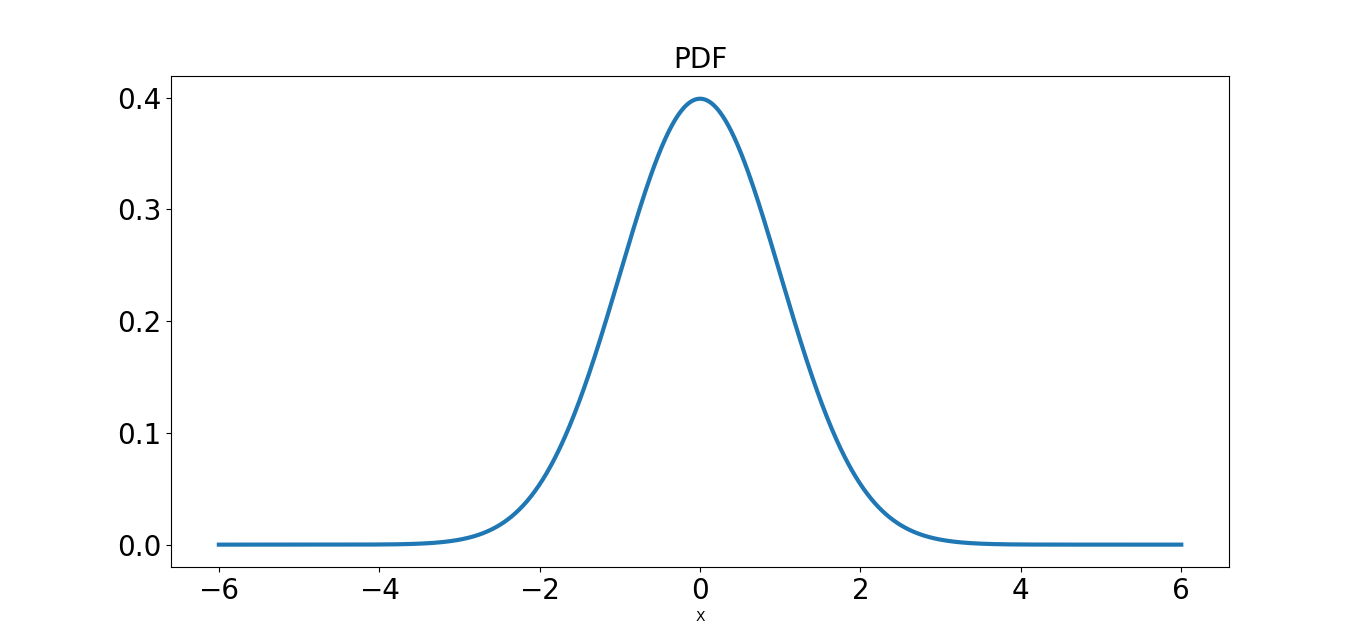
\includegraphics[width=80mm]{pdf_quiz6.png}
\end{subfigure}
\begin{subfigure}{0.49\textwidth}
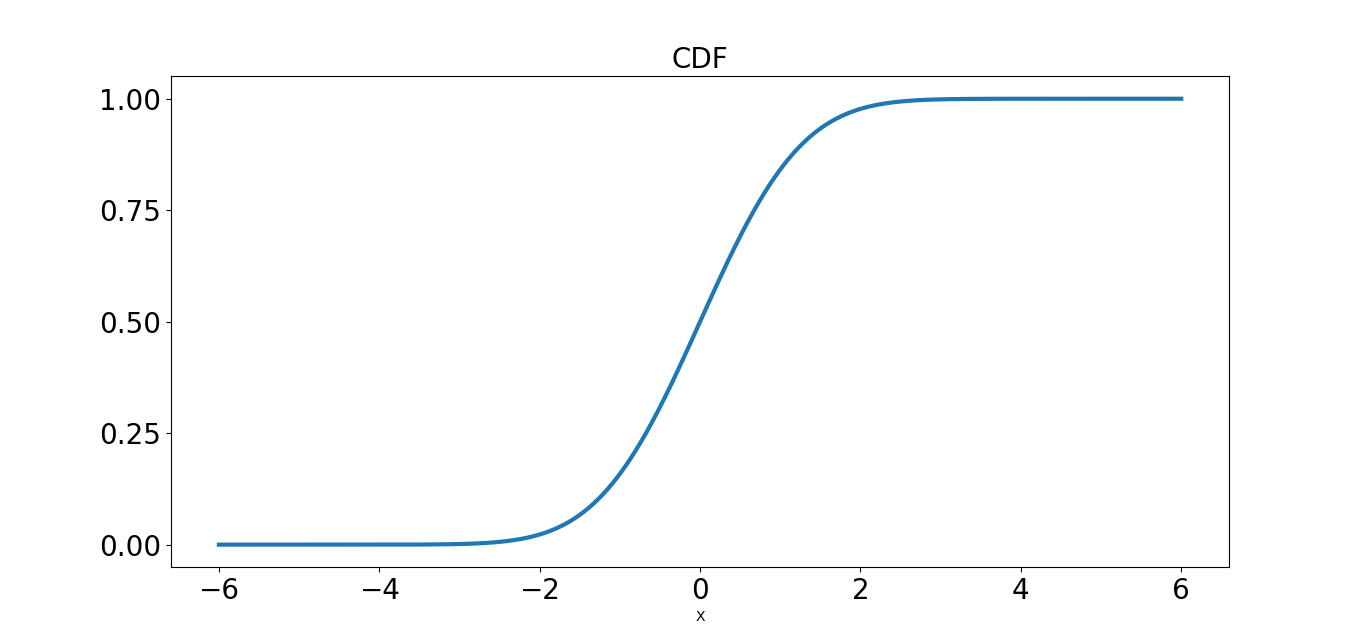
\includegraphics[width=80mm]{cdf_quiz6.png}
\end{subfigure}
\end{figure}

اگر چگالی احتمال و توزیع تجمعی متغیر $Y=2-X$ را بر حسب چگالی احتمال و توزیع تجمعی متغیر $X$ بیابید و آنها را رسم کنید.

\Q
از دو جامعه ی آماری بزرگ، یک آزمون علمی 100 نمره ای گرفته شده است. مشاهده شده که نمرات افراد این دو جامعه، به ترتیب از دو توزیع گوسی با میانگین های 59 و 73 و واریانس های 9 و 16 پیروی می کند.

الف) کدام یک از این دو جامعه به طور متوسط دارای سطح علمی بالاتری است؟ چرا؟

ب) افراد کدام جامعه دارای سطح علمی نزدیک تری به یکدیگر هستند؟ (یا به عبارت دیگر، هم سطح ترند؟) چرا؟

\Q
الف) آیا چگالی احتمال یک متغیر تصادفی می تواند تابعی فرد باشد؟ توضیح دهید.

ب) گشتاور مرتبه $n$-ام یک متغیر تصادفی یکنواخت در بازه‌ی $[a,b]$ را به دست آورید.

\Q
الف) برای هر متغیر تصادفی $X$ و $s>0$ تحقیق کنید 
$$
\Pr\{X\ge a\}=\Pr\{e^{sX}\ge e^{sa}\}
$$
ب) به کمک نامساوی مارکوف ثابت کنید:
$$
\Pr\{X\ge x\}\le e^{-sx}\Phi_X(s)
$$

\Q
تعیین کنید به ازای چه مقادیری از $k$، هر یک از توابع زیر می تواند تابع توزیع تجمعی یک متغیر تصادفی باشد.

الف) 
$
F(x)=\begin{cases}
1-e^{-kx^2}&,\quad x\ge 0\\
0&,\quad x<0
\end{cases}
$
\quad,\quad
ب)
$
F(x)={e^x\over e^x+k}
$

پ)
$
F(x)=\begin{cases}
kx&,\quad 0\le x\le 1\\
1&,\quad x>1\\
0&,\quad x<0
\end{cases}
$
\quad,\quad
ت)
$
F(x)=\cos {\pi\over e^x+k}
$

ث)
$
F(x)=\begin{cases}
k-e^{x-x^2}&,\quad x\ge 0\\
0&,\quad x<0
\end{cases}
$

\Q
اگر $F(x)$ تابع توزیع تجمعی یک متغیر تصادفی پیوسته باشد، کدام یک از توابع زیر می‌توانند تابع توزیع تجمعی یک متغیر تصادفی باشند؟ سپس برای هر تابع توزیع تجمعی، مقدار 
$\Pr\{1<X\le 2\}$
را بیابید (راهنمایی: از خواص تابع توزیع تجمعی بهره بگیرید.).

الف) 
$
F(x^2)
$
\quad,\quad
ب) 
$
F(x^3)
$
\quad,\quad
پ) 
$
1-F(-x)
$
\quad,\quad
ت) 
$
F^n(x)
$
برای هر مقدار طبیعی از $n$
\quad,\quad
ث) 
$
\sin\left[{\pi\over 2}F(x)\right]
$

\Q
تعیین کنید به ازای چه مقادیری از $k$، هر یک از توابع زیر می تواند چگالی احتمال یک متغیر تصادفی باشد. سپس برای هر چگالی احتمال، مقادیر 
$\Pr\{X=1\}$
و
$\Pr\left\{X<{1\over 2}\right\}$
را بیابید.

الف) 
$
f(x)=\begin{cases}
1/x^k&,\quad x\ge 1\\
0&,\quad x<0
\end{cases}
$
\quad,\quad
ب)
$
f(x)=\begin{cases}
kxe^{-x}&,\quad x\ge 0\\
0&,\quad x<0
\end{cases}
$

پ)
$
f(x)=\begin{cases}
\sin x&,0\le x\le k\\
0&,\quad \text{سایر جاها}
\end{cases}
$
\quad,\quad
ت)
$
f(x)=k\delta(x-1)+(1-k)\delta(x)
$

ث)
$
f(x)=\begin{cases}
k\delta(x-1)&,\quad x=1\\
x&,\quad 0<x<1\\
0&,\quad \text{سایر جاها}
\end{cases}
$
(به عبارت دیگر، تابع در نقطه‌ی $x=1$ دارای ضربه‌ای به مساحت $k$ است)



\Q
یک سامانه دارای 70 قطعه است. پیشامد اینکه هر قطعه پس از شروع به کار در زمان 0، در بازه‌ی 
$
(0,x)
$
دچار خرابی گردد، یک متغیر تصادفی با چگالی احتمال زیر است:
$$
f(x)=\begin{cases}
{1\over T}e^{-{x\over T}}&,\quad x\ge 0\\
0&,\quad x<0
\end{cases}
$$
احتمال آن را بیابید که بیش از 65 قطعه از این سیستم در بازه‌ی 
$
\left(0,{T\over 4}\right)
$
 دچار خرابی نشوند.

\Q
اگر 
$x_u$،
صدک-$u$ متغیر تصادفی 
$X$
باشد، در این صورت مقدار 
$x_u$
را به ازای 
$u=0.2,0.4,0.6,0.8$
برای توابع چگالی احتمال زیر به دست آورید.

الف)
$
f(x)=\begin{cases}
1&,\quad 0\le x\le 1\\
0&,\quad \text{سایر جاها}
\end{cases}
$
\quad,\quad
ب)
$
f(x)=\begin{cases}
2e^{-2x}&,\quad x\ge 0\\
0&,\quad \text{سایر جاها}
\end{cases}
$

\Q
زمان خرابی یک لامپ، یک متغیر تصادفی با چگالی احتمال زیر است،
$$
f_X(x)={1\over\lambda}e^{-{x\over\lambda}}\quad,\quad x>0
$$

الف) احتمال آن که این لامپ، به مدت حداکثر
$
2\lambda
$
عمر کند، چقدر است؟

ب) احتمال آن که این لامپ بیش از 
$
3\lambda
$
و کمتر از 
$
3.5\lambda
$
عمر کند چقدر است؟

\Q
یک متغیر تصادفی دارای چگالی احتمال زیر است،
$$
f_X(x)=\begin{cases}
6x^2(1-x)&,\quad 0\le x\le1\\
k\delta(x+1)&,\quad x=-1\\
0&,\quad \text{سایر جاها}
\end{cases}
$$
به عبارت دیگر، چگالی احتمال دارای ضربه ای به اندازه $k$ در $x=-1$ است.

الف) مقدار $k$ را بیابید.

ب) تابع توزیع تجمعی را به دست آورید و آن را رسم کنید.

پ) مقدار احتمال های 
$\Pr\{-2< X\le {1\over2}\}$
و
$\Pr\{0< X\le {1\over2}\}$
چقدر است؟

\Q
فرض کنید متغیر تصادفی $X$ دارای توزیع یکنواخت بین 0 و 1 است. در این صورت، تابع توزیع تجمعی و چگالی احتمال هر یک از متغیرهای تصادفی زیر را بیابید. سپس، مقادیر احتمال های 
$\Pr\{X\le {2\over 3}\}$
و
$\Pr\{Y\le {1\over \sqrt3}\}$
را از روی چگالی‌های احتمال $X$ و $Y$ بیابید و با هم مقایسه کنید. نتیجه مقایسه را توضیح دهید.


الف)
$
Y=X^2
$
\quad,\quad
ب)
$
Y=-\ln (1-X)
$
\quad,\quad
پ)
$
Y=\tan\pi (X-{1\over 2})
$

\Q
اگر تابع توزیع تجمعی متغیر تصادفی $X$ را با $F(x)$ نشان دهیم، توابع توزیع تجمعی متغیرهای تصادفی زیر را برحسب $F(x)$ دست آورید.

الف)
$Y=|X|$
\quad,\quad
ب)
$
Y=\begin{cases}
0&,\quad X\le0\\
1&,\quad X>0
\end{cases}
$
\quad,\quad
پ)
$Y=X^2-2X$

\Q
تابع جرم احتمال متغیر تصادفی $X$ دارای خاصیت زیر است:
$$6\Pr\{X=k+2\}-5\Pr\{X=k+1\}+\Pr\{X=k\}=0\quad,\quad k=1,2,\cdots$$
همچنین 
$\Pr\{X=1\}=\frac{7}{12}$.
در این صورت، چگالی جرم احتمال متغیر $X$ را بیابید.

\Q
متغیر تصادفی $X$ دارای چگالی احتمال زیر است:
$$f(x)=\frac{a}{2}e^{-ax}+\frac{1}{2}e^{-x}\quad,\quad x>0.$$
مقدار $a$ را به گونه ای بیابید به طوری که
$\mathbb{E}\{X\}=5$.

\Q
برای هر یک از توابع زیر، محدوده مقادیر $k$ را به گونه ای تعیین کنید که تابع مورد نظر، یک تابع توزیع انباشته باشد. سپس، چگالی احتمال را بیابید.

الف)
$F(x)=\frac{1}{e^{-kx}+1}$
\quad,\quad
ب)
$
F(x)=\begin{cases}
0&,\quad x<0\\
1-e^{-x-k\sin x}&,\quad x\ge0
\end{cases}
$

پ)
$
F(x)=\begin{cases}
0&,\quad x<0\\
1+xe^{-kx}&,\quad x\ge 0
\end{cases}
$

ت)
$
F(x)=\begin{cases}
0&,\quad x<0\\
\frac{1}{2}&,\quad 0\le x<1\\
1-\frac{1}{2}e^{k-kx}&,\quad x\ge 1
\end{cases}
$

\Q
برای بخش های الف و ت سوال پیش، مقادیر میانه، صدکهای 25ام و 75ام و همچنین احتمال‌های
$\Pr\{X=0\}$
و
$\Pr\{0< X\le 2\}$
را بیابید.

\Q
یک تاس را پرتاب می‌کنیم. اگر زوج آمد، عدد آن را یادداشت می‌کنیم و اگر فرد آمد، عددی را به تصادف از بازه‌ی 
$[1,6]$
انتخاب کرده و آن را یادداشت می‌کنیم. اگر متغیر تصادفی 
$X$،
نشان دهنده‌ی عدد یادداشت شده باشد، چگالی احتمال و تابع توزیع انباشته‌ی آن را به دست آورده و رسم کنید. سپس، مقدار 
$\Pr\{1\le X\le 3\}$
را بیابید.



\Q
فرض کنید متغیر تصادفی $X$، از توزیع نمایی با پارامتر $\lambda=1$ پیروی کند. در این صورت، چگالی احتمال متغیر تصادفی $Y$ را در حالت های زیر بیابید.

الف)
$
Y=e^X
$
\quad,\quad
ب)
$
Y=X^\alpha
$
که
$
\alpha
$
عدد ثابت مثبتی است.

پ)
$
Y=\lfloor X\rfloor
$

\Q
فرض کنید $X$، یک متغیر تصادفی باشد که از توزیع زیر پیروی می‌کند:
$$
f_X(x)=\begin{cases}
kx&,\quad 0<x<1\\
\frac{1}{2}\delta(x)&,\quad x=1\\
0&,\quad \text{جاهای دیگر}
\end{cases}
$$

الف) مقدار مناسب $k$ را بیابید.
\quad,\quad
ب) مقدار 
$
\mathbb{E}\{X\}
$
را محاسبه کنید.

پ) مقدار 
$
\mathbb{E}\{e^{aX}\}
$
را به دست آورید که $a$ عدد حقیقی دلخواهی است.

\Q
متغیر تصادفی $X$ از توزیع زیر پیروی می‌کند:
$$
f_X(x)=\begin{cases}
2xe^{-x^2}&,\quad x>0\\
0&,\quad \text{جاهای دیگر}\\
\end{cases}
$$
متغیر تصادفی
$
Y=X^2
$
مفروض است.

الف) چگالی احتمال $Y$ را به دست آورید.
\quad,\quad
ب) امید ریاضی $X$ را بیابید.

پ) امید ریاضی $Y$ را از روی چگالی احتمال آن و مقدار 
$
\mathbb{E}\{X^2\}
$
را از قضیه‌ی اساسی امید ریاضی محاسبه کرده و با هم مقایسه کنید.

ت) مقادیر
$
\Pr\{X<\frac{1}{2}\}
$
و
$
\Pr\{Y<\frac{1}{4}\}
$
را به ترتیب از روی چگالی های احتمال 
$
X
$
و
$
Y
$
به دست آورده و با هم مقایسه کنید.

\Q
برای هر یک از توزیع های زیر، مقدار 
$
\Pr\{X\ge \alpha\}
$
را به دست آورده و همچنین، یک کران بالا برای این احتمال برای هر توزیع با کمک نامساوی مارکوف به دست آورید. سپس مقدار دقیق احتمال و کران آن را مقایسه کنید.

الف)
$
f(x)=e^{-x}\quad,\quad x>0
$
\quad,\quad
ب)
$
f(x)=\frac{1}{\ln 2}\frac{1}{1+e^x}\quad,\quad x>0
$

پ)
$
f(x)=xe^{-x}\quad,\quad x>0
$

\Q
برای توزیع‌های بخش های الف و پ سوال پیش، مقدار واریانس را به دست آورید.

\Q
برای هر یک از توزیع های زیر، تابع مولد گشتاور را یافته و سپس از روی آن، مقدار 
$
\mathbb{E}\{X^2\}
$
را بیابید.

الف)
$
f(x)=\begin{cases}
1-x&,\quad 0<x<1\\
\frac{1}{2}\delta(x-1)&,\quad x=1
\end{cases}
$

ب)
$
f(x)=\begin{cases}
\cos x&,\quad 0<x<\frac{\pi}{2}\\
0&,\quad \text{جاهای دیگر}
\end{cases}
$

پ)
$
\Pr\{X=x\}=
\begin{cases}
\frac{n}{2^{n+1}}&,\quad n\in\Bbb N\\
0&,\quad \text{جاهای دیگر}
\end{cases}
$

ت)
$
X
$
متغیر تصادفی حاصل ضرب دو عدد رو آمده در پرتاب دو تاس به طور مستقل است.

\Q
برای هر یک از متغیرهای تصادفی زیر، واریانس را به دست آورید.

الف) 
$
f_X(x)=\begin{cases}
e^{-x}&,\quad x>1\\
0&,\quad x\le1
\end{cases}
$

ب) 
$
f_X(x)=\begin{cases}
\sin x&,\quad 0<x<{\pi\over 2}\\
0&,\quad \text{سایر جاها}
\end{cases}
$

پ)
$
f_X(x)=
\begin{cases}
{2\over x^3}&,\quad x>1\\
0&,\quad \text{سایر جاها}
\end{cases}
$

ت) X یک متغیر تصادفی گسسته است و 
$
\Pr\{X=i\}=2({1\over 3})^i
$
برای 
$
i\in\Bbb N
$

\Q
برای قسمت های الف و ت سوال 1، ابتدا تابع مولد گشتاور را محاسبه نموده و سپس از روی آن، میانگین و واریانس را به دست آورید.

\Q
برای قسمت های الف و ب سوال 1، میانگین متغیر تصادفی $e^{-X}$ را بیابید.

\Q
برای متغیر تصادفی $X$ با چگالی‌های احتمال زیر، ابتدا تابع مولد گشتاور را یافته و سپس از روی آن، مقادیر میانگین، واریانس و 
$\text{var}\left\{X|X>\frac{1}{2}\right\}$
 را بیابید.

الف)
$
f_X(x)=\begin{cases}
{1\over 2}\sin x&,\quad 0<x<\pi\\
0&,\quad \text{سایر جاها}
\end{cases}
$

ب)
$
f_X(x)=\begin{cases}
\cos x&,\quad 0<x<{\pi\over 2}\\
0&,\quad \text{سایر جاها}
\end{cases}
$

پ)
$
f_X(x)=\begin{cases}
xe^{-x}&,\quad x>0\\
0&,\quad \text{سایر جاها}
\end{cases}
$

ت)
$
f_X(x)=\begin{cases}
\frac{3}{7}x^2&,\quad 1<x<2\\
0&,\quad \text{سایر جاها}
\end{cases}
$

ث)
$
f_X(x)=\begin{cases}
\frac{1}{2}\delta(x-1)&,\quad x=1\\
x&,\quad 0<x<1\\
0&,\quad \text{سایر جاها}
\end{cases}
$